% !TEX program = xelatex
\documentclass[UTF8,fontset=fandol,a4paper,11pt]{ctexart}
\usepackage[margin=21mm,top=23mm,bottom=22mm,headheight=16pt]{geometry}
\usepackage{amsmath,amssymb,mathtools,bm}
\usepackage{tikz}
\usetikzlibrary{arrows.meta,calc,angles,quotes,patterns}
\usepackage{xcolor,booktabs,array,longtable,enumitem,fancyhdr,needspace}
\usepackage[unicode,hidelinks]{hyperref}
\definecolor{ink}{HTML}{24343C}
\definecolor{accent}{HTML}{166A70}
\definecolor{muted}{HTML}{65747A}
\definecolor{rulegray}{HTML}{D4DDE0}
\definecolor{warm}{HTML}{966037}
\color{ink}
\setlength{\parindent}{2em}
\setlength{\parskip}{4pt}
\linespread{1.12}
\AtBeginDocument{\setlength{\abovedisplayskip}{6pt plus 2pt minus 1pt}
\setlength{\belowdisplayskip}{6pt plus 2pt minus 1pt}
\setlength{\abovedisplayshortskip}{0pt plus 1pt}
\setlength{\belowdisplayshortskip}{4pt plus 1pt}}
\setlist[enumerate]{label=(\arabic*),leftmargin=2.3em,itemsep=3pt,topsep=4pt}
\setlist[itemize]{leftmargin=2em,itemsep=2pt,topsep=4pt}
\allowdisplaybreaks[1]
\setlength{\emergencystretch}{2em}
\setcounter{secnumdepth}{0}
\providecommand{\tightlist}{\setlength{\itemsep}{0pt}\setlength{\parskip}{0pt}}
\ctexset{section={format=\Large\bfseries\color{accent},beforeskip=10pt,afterskip=9pt},
subsection={format=\normalsize\bfseries\color{accent},beforeskip=10pt,afterskip=4pt},
subsubsection={format=\normalsize\bfseries,beforeskip=8pt,afterskip=3pt}}
\pagestyle{fancy}
\fancyhf{}
\fancyhead[L]{\small\color{muted}物理学难题集萃}
% 页眉仅保留书名；版本名称只在封面显示。
\fancyfoot[L]{\small\color{muted}\chapterlabel}
\fancyfoot[R]{\small\thepage}
\renewcommand{\headrulewidth}{0.4pt}
\renewcommand{\footrulewidth}{0pt}
\newcommand{\dd}{\mathop{}\!\mathrm{d}}
\newcommand{\vect}[1]{\bm{#1}}
\newcommand{\tagline}[1]{\noindent{\small\color{muted}#1}\par}
\newcommand{\result}[1]{\begin{equation*}\boxed{#1}\end{equation*}}
\newcommand{\figcaption}[1]{\par\vspace{2pt}{\small\color{muted}#1}\par}
\newcommand{\teach}[2]{\Needspace{4\baselineskip}\subsection*{讲解要点与追问}#1\par\smallskip\noindent\textbf{追问：}#2\par}
\newcommand{\workarea}{\par\vspace{7mm}\noindent{\small\color{muted}作答区}\par\vspace{4mm}
\noindent\textcolor{rulegray}{\rule{\linewidth}{0.3pt}}\par\vspace{16mm}
\noindent\textcolor{rulegray}{\rule{\linewidth}{0.3pt}}\par\vspace{16mm}
\noindent\textcolor{rulegray}{\rule{\linewidth}{0.3pt}}\par\vspace{16mm}
\noindent\textcolor{rulegray}{\rule{\linewidth}{0.3pt}}}
\tikzset{axis/.style={-{Stealth[length=2mm]},thin,color=muted},
motion/.style={-{Stealth[length=2.3mm]},thick,color=accent},
force/.style={-{Stealth[length=2.3mm]},thick,color=warm},
traj/.style={thick,color=accent},guide/.style={dashed,thin,color=muted},
object/.style={thick,color=ink},every node/.style={font=\small}}\widowpenalty=10000\clubpenalty=10000\displaywidowpenalty=10000

\newcommand{\chapterlabel}{热学第二章\quad 热力学第一、第二定律}
\hypersetup{pdftitle={热学第二章 热力学第一、第二定律·学生版},pdfauthor={},pdfsubject={热学第二章第1--25题}}
\begin{document}
\pdfbookmark[0]{热学第二章 热力学第一、第二定律}{cover}
\thispagestyle{empty}\vspace*{20mm}
\noindent{\Huge\bfseries 物理学难题集萃}\par\vspace{8mm}
\noindent{\LARGE 热学第二章}\par\vspace{5mm}
\noindent{\LARGE 热力学第一、第二定律}\par\vspace{10mm}
\noindent{\Large\color{accent}学生版}\par\vspace{8mm}
\noindent\textcolor{accent}{\rule{\linewidth}{1pt}}\par\vspace{8mm}
\noindent 第1--25题\par\vspace{5mm}
\noindent 题目、题图与作答区。\par\vfill\clearpage
\pdfbookmark[1]{题目目录}{contents}\section*{题目目录}
\begin{longtable}{@{}>{\color{accent}\bfseries}r p{120mm}@{}}
\toprule 题号 & 题目\\\midrule
1 & 循环过程证明比热不可能恒定 \\
2 & 平移等温线确定过程比热曲线 \\
3 & 直线过程的温度图像与比热正负 \\
4 & 单原子双原子混合理想气体的绝热指数 \\
5 & 热功效率恒定过程中的总功 \\
6 & 变热容量过程的内能增量与作功 \\
7 & 钢丝棉氧化反应中的热量与内能变化 \\
8 & 双活塞气缸加热的分段末温 \\
9 & 绝热压缩后缓慢扩散的终温 \\
10 & 带阀绝热活塞与电热器的能量分配 \\
11 & 绝热左筒与等温右筒的活塞平衡 \\
12 & 带阀隔板气缸的分段绝热压缩功 \\
13 & 绝热容器中推活塞后混合的终压 \\
14 & 潮湿空气越山降雨的热力学估算 \\
15 & U形管水银振动与封闭空气绝热弹性 \\
16 & 由声速驻波判断碘蒸气分子类型 \\
17 & 两个三角循环效率的比较 \\
18 & 多条过程线构成循环的效率比较 \\
19 & 氦气三直线循环效率 \\
20 & 直线加绝热线循环的效率与极值温度 \\
21 & 圆形准静态循环的功、热量和转折点 \\
22 & 可逆卡诺空调的维持室温与最高外温 \\
23 & 绝热细棒热平衡过程的熵增 \\
24 & 氧气复合循环效率与 S-T 图像 \\
25 & 由 T-S 直线导出理想气体过程方程 \\\bottomrule\end{longtable}

\clearpage

\pdfbookmark[2]{第 1 题 循环过程证明比热不可能恒定}{q1}

\section*{第 1 题\quad 循环过程证明比热不可能恒定}

一定量理想气体经历图示顺时针准静态循环，$p-V$图中闭合曲线围成的面积不为零。以$\delta Q=M c\dd T$定义沿过程的质量比热，$M$为气体质量。证明该循环的过程比热$c$不可能处处为同一个有限常量，并讨论循环反向时的结论。

\begin{center}\begin{minipage}{0.96\linewidth}\centering
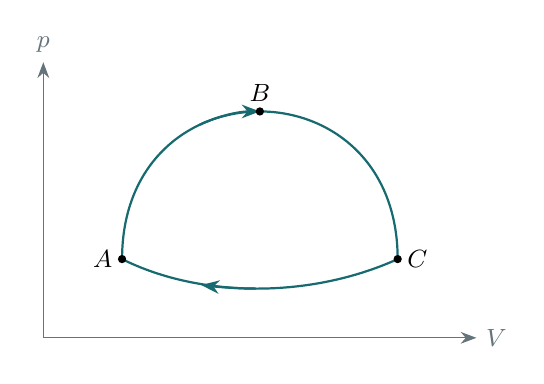
\begin{tikzpicture}[x=1cm,y=1cm,font=\small]
\draw[axis] (0,0)--(5.5,0) node[right] {$V$};
\draw[axis] (0,0)--(0,3.5) node[above] {$p$};
\draw[traj] (1,1) .. controls (1,3.5) and (4.5,3.5) .. (4.5,1)
 .. controls (3.4,.5) and (2,.5) .. (1,1);
\draw[motion] (1.986125,2.70625) .. controls (2.225,2.82) and (2.49,2.875) .. (2.75,2.875);
\draw[motion] (2.705,.625) .. controls (2.48,.625) and (2.23,.645) .. (2.006,.67);
\fill (1,1) circle(1.5pt) node[left] {$A$};
\fill (2.75,2.875) circle(1.5pt) node[above] {$B$};
\fill (4.5,1) circle(1.5pt) node[right] {$C$};
\end{tikzpicture}\figcaption{图 热2.1　闭合路径包围非零面积；箭头给出循环方向。}\end{minipage}\end{center}

\workarea

\clearpage

\pdfbookmark[2]{第 2 题 平移等温线确定过程比热曲线}{q2}

\section*{第 2 题\quad 平移等温线确定过程比热曲线}

质量为$M$、摩尔质量为$\mu$的理想气体，定容比热$c_V$为常量。其准静态过程$x$在$p-V$平面上向下平移$p_0>0$后，恰成为温度$T_0$的等温线。求过程$x$的温度下限及其在曲线上的位置；导出$c$与$p$的关系，画出$c-p$曲线。

\begin{center}\begin{minipage}{0.96\linewidth}\centering
\begin{tikzpicture}[x=1cm,y=1cm,font=\small]\draw[axis] (0,0)--(5.5,0) node[right] {$V$};\draw[axis] (0,0)--(0,3.5) node[above] {$p$};
\draw[traj,domain=.65:5,samples=60] plot (\x,{1+1.6/\x});\draw[guide,domain=.65:5,samples=60] plot (\x,{1.6/\x});\draw[<->] (3,.533)--(3,1.533) node[right,midway]{$p_0$};\node[right] at (4.7,1.5) {$x$};\node[right] at (3.7,.25) {$T=T_0$};
\end{tikzpicture}\figcaption{图 热2.2　实线向下平移$p_0$成为等温虚线，同一体积处比较压强。}\end{minipage}\end{center}

\workarea

\clearpage

\pdfbookmark[2]{第 3 题 直线过程的温度图像与比热正负}{q3}

\section*{第 3 题\quad 直线过程的温度图像与比热正负}

质量为$M$、摩尔质量为$\mu$的理想气体，定容比热$c_V=3R/(2\mu)$。气体沿直线由$A(V_0,2p_0)$到$B(2V_0,p_0)$。求$T(V)$并作图；求过程比热$c(V)$并作图，结合$\delta Q/(M\dd T)$解释各段$c$的正负。

\begin{center}\begin{minipage}{0.96\linewidth}\centering
\begin{tikzpicture}[x=1cm,y=1cm,font=\small]\draw[axis] (0,0)--(5.5,0) node[right] {$V/V_0$};\draw[axis] (0,0)--(0,3.5) node[above] {$p/p_0$};
\draw[traj] (1,2)--(2,1);\draw[motion] (1.25,1.75)--(1.65,1.35);\fill[ink] (1,2) circle(1.4pt);\node[above right] at (1,2) {A};
\fill[ink] (2,1) circle(1.4pt);\node[above right] at (2,1) {B};
\draw[guide] (1,0) node[below]{1}--(1,2)--(0,2) node[left]{2};\draw[guide] (2,0) node[below]{2}--(2,1)--(0,1) node[left]{1};
\end{tikzpicture}\figcaption{图 热2.3　直线连接两端状态；坐标按$V_0,p_0$归一化。}\end{minipage}\end{center}

\workarea

\clearpage

\pdfbookmark[2]{第 4 题 单原子双原子混合理想气体的绝热指数}{q4}

\section*{第 4 题\quad 单原子双原子混合理想气体的绝热指数}

由$\nu_1$ mol单原子气体和$\nu_2$ mol双原子气体组成的理想混合气体，在常温下的准静态绝热方程为$pV^{11/7}=\text{常量}$。忽略双原子分子的振动自由度，求摩尔数比$\alpha=\nu_1/\nu_2$。

\begin{center}\begin{minipage}{0.96\linewidth}\centering
\begin{tikzpicture}[x=1cm,y=1cm,font=\small]\draw[object,fill=accent!6] (0,0) rectangle (6,1.8);\draw[guide] (3,0)--(3,1.8);\node[align=center] at (1.5,.9) {$\nu_1$ mol\\单原子};\node[align=center] at (4.5,.9) {$\nu_2$ mol\\双原子};\node[above] at (3,2.1){两组分混合，温度共同为$T$};
\end{tikzpicture}\figcaption{图 热2.4　图中虚线区分两组分的名称；两种分子均分布在总容积中。}\end{minipage}\end{center}

\workarea

\clearpage

\pdfbookmark[2]{第 5 题 热功效率恒定过程中的总功}{q5}

\section*{第 5 题\quad 热功效率恒定过程中的总功}

1 mol单原子理想气体经历准静态过程，初态$(4p_0,V_0)$，终态$(p_0/4,8V_0)$。每一微小过程的热功比$\delta W/\delta Q$均相同。求全过程气体对外所作的功$W$。

\begin{center}\begin{minipage}{0.96\linewidth}\centering
\begin{tikzpicture}[x=1cm,y=1cm,font=\small]\draw[axis] (0,0)--(5.5,0) node[right] {$V/V_0$};\draw[axis] (0,0)--(0,3.5) node[above] {$p/p_0$};
\draw[traj,domain=1:8,samples=70] plot ({.6*\x},{.75*4/pow(\x,4/3)});\fill[ink] (0.6,3) circle(1.4pt);\node[above right] at (0.6,3) {初态 $(1,4)$};
\fill[ink] (4.8,0.1875) circle(1.4pt);\node[above right] at (4.8,0.1875) {末态 $(8,1/4)$};

\end{tikzpicture}\figcaption{图 热2.5　曲线满足微元热功比恒定；图中横纵比例不同。}\end{minipage}\end{center}

\workarea

\clearpage

\pdfbookmark[2]{第 6 题 变热容量过程的内能增量与作功}{q6}

\section*{第 6 题\quad 变热容量过程的内能增量与作功}

2 mol单原子理想气体经历总过程热容量$C(T)=2R(1+bT)$的准静态过程，$b=0.01\,\mathrm{K^{-1}}$。终温为初温的2倍，终体积为初体积的$\sqrt2$倍。求内能增量$\Delta U$及气体对外作功$W$。

\begin{center}\begin{minipage}{0.96\linewidth}\centering
\begin{tikzpicture}[x=3.5cm,y=.7cm]
\draw[axis] (0,0)--(1.75,0) node[right] {$u=bT$};
\draw[axis] (0,0)--(0,5.7) node[above] {$C/R$};
\draw[traj,domain=0:1.55,samples=60] plot (\x,{2*(1+\x)});
\draw[guide] (0,3) node[left] {$3$}--(1.6,3) node[right] {$C_V^{\rm total}/R=3$};
\node[left] at (0,2) {$2$};
\draw[guide] (.6931471806,0) node[below] {$\ln2$}--(.6931471806,3.3862943611);
\draw[guide] (1.3862943611,0) node[below] {$2\ln2$}--(1.3862943611,4.7725887222);
\fill (.6931471806,3.3862943611) circle(1.5pt) node[above left] {$A$};
\fill (1.3862943611,4.7725887222) circle(1.5pt) node[above left] {$B$};
\end{tikzpicture}\figcaption{图 热2.6　按$u=bT$和$C/R$标定；实线有非零截距，虚线给整份气体的定容热容量。}\end{minipage}\end{center}

\workarea

\clearpage

\pdfbookmark[2]{第 7 题 钢丝棉氧化反应中的热量与内能变化}{q7}

\section*{第 7 题\quad 钢丝棉氧化反应中的热量与内能变化}

空气中氮气、氧气的质量分数分别为76.9\%、23.1\%，其余成分忽略。气缸内装有空气和钢丝棉，活塞无摩擦地移动，使气压保持$1\,\mathrm{atm}$。在$300\,\mathrm K$下缓慢反应，生成1 mol $\mathrm{Fe_2O_3}$后，氧气恰耗尽；全过程向外释放$8.24\times10^5\,\mathrm J$热量。求系统内能变化、缸内气体内能变化和氮气密度变化。系统包括全部气体、铁及氧化物；固体体积忽略，氧气和氮气每摩尔内能均为$5RT/2$。

\begin{center}\begin{minipage}{0.96\linewidth}\centering
\begin{tikzpicture}[x=1cm,y=1cm]
\foreach \x/\h in {0/2.5256827048,5/2}{
 \fill[accent!7] (\x,0) rectangle ++(2.2,\h);
 \draw[object] (\x,3.15)--(\x,0)--++(2.2,0)--++(0,3.15);
 \draw[object,line width=2pt] (\x,\h)--++(2.2,0);
}
\node[align=center] at (1.1,1.3) {$\mathrm{N_2,O_2}$\\$V_i$};
\node[align=center] at (6.1,1.3) {$\mathrm{N_2}$\\$V_f\simeq0.792V_i$};
\node at (1.1,.25) {钢丝棉};
\node[align=center] at (6.1,.5) {$\mathrm{Fe_2O_3}$\\可有剩余铁};
\draw[guide] (5,2.5256827048)--(7.2,2.5256827048);
\draw[motion] (2.55,1.3)--(4.65,1.3);
\node[above,align=center] at (3.6,1.6) {恒温恒压\\反应};
\node[above] at (1.1,3.2) {初态};
\node[above] at (6.1,3.2) {末态};
\end{tikzpicture}\figcaption{图 热2.7　同一气缸的初、末状态分别画出；气相体积减小，钢丝棉只作符号示意。}\end{minipage}\end{center}

\workarea

\clearpage

\pdfbookmark[2]{第 8 题 双活塞气缸加热的分段末温}{q8}

\section*{第 8 题\quad 双活塞气缸加热的分段末温}

固定直立气缸由相连通的上下圆筒构成。上筒容积$V_m$，其中薄活塞A质量$2m$、面积$2S$；足够长的下筒有活塞B，质量$m$、面积$S$。A上方有1 mol理想气体，A、B之间有另一气体，B下方与压强$p_0$的大气连通。两活塞无摩擦、不漏气；筒壁、短连接管和活塞均绝热。初态平衡，A上方温度$T_0$，每摩尔内能$U=CT$，$C$为常量。通过顶部电热丝向A上方气体缓慢输入热量$Q_0\ge0$，求终态温度$T_f$，讨论A是否到达上筒底端的各种情况。取$p_0>2mg/S$。

\begin{center}\begin{minipage}{0.96\linewidth}\centering
\begin{tikzpicture}[x=1cm,y=1cm,font=\small]\draw[object] (0,4)--(0,1.8)--(.6,1.8)--(.6,0);\draw[object] (2,4)--(2,1.8)--(1.6,1.8)--(1.6,0);\draw[object] (0,4)--(2,4);\fill[accent!8] (0,2.6) rectangle(2,4);\draw[object,line width=2pt] (0,2.6)--(2,2.6);\draw[object,line width=2pt] (.6,.7)--(1.6,.7);\node at (1,3.3){$T,V$};\node[right] at (2.15,2.6){A：$2m,2S$};\node[right] at (2.15,.7){B：$m,S$};\node[below] at (1,0){大气$p_0$};\draw[force] (1,4.6)--(1,3.8) node[pos=0,left]{$Q_0$};
\end{tikzpicture}\figcaption{图 热2.8　A向下移动使其上方气体膨胀，A到上筒底端后体积固定。}\end{minipage}\end{center}

\workarea

\clearpage

\pdfbookmark[2]{第 9 题 绝热压缩后缓慢扩散的终温}{q9}

\section*{第 9 题\quad 绝热压缩后缓慢扩散的终温}

两个对外绝热容器A、B经短细管相连，阀门K导热良好，活塞F绝热、无摩擦、不漏气；装置热容量忽略。初始K关，A内有$n$ mol理想气体，温度$T_0$，B为真空。推F将A中气体压缩到与B容积相等，外界作功$W$，温度升为$T_1$。再稍开K，使气体缓慢流入B，同时缓慢推F，保持F附近气压近似不变。直到两容器达到共同平衡，求终温。气体定容摩尔热容量为常量。

\begin{center}\begin{minipage}{0.96\linewidth}\centering
\begin{tikzpicture}[x=1cm,y=1cm]
\fill[accent!7] (.4,0) rectangle (3.4,1.8);
\draw[object] (-.6,1.8)--(3.4,1.8)--(3.4,1.05);
\draw[object] (-.6,0)--(3.4,0)--(3.4,.75);
\draw[object] (4.4,1.05)--(4.4,1.8)--(7.4,1.8)--(7.4,0)--(4.4,0)--(4.4,.75);
\draw[object] (3.4,.75)--(4.4,.75) (3.4,1.05)--(4.4,1.05);
\draw[object,line width=2pt] (.4,0)--(.4,1.8);
\draw[object] (-1.2,.9)--(.4,.9);
\node[above] at (-.8,.9) {$F$};
\draw[object] (3.9,.75)--(3.9,1.05);
\node[above] at (3.9,1.15) {$K$};
\node[align=center] at (1.9,.9) {$A$\\$n,T_1,V_1$};
\node[align=center] at (5.9,.9) {$B$\\真空，$V_1$};
\end{tikzpicture}\figcaption{图 热2.9　第一阶段结束后，A、B几何容积相等，B仍为真空。}\end{minipage}\end{center}

\workarea

\clearpage

\pdfbookmark[2]{第 10 题 带阀绝热活塞与电热器的能量分配}{q10}

\section*{第 10 题\quad 带阀绝热活塞与电热器的能量分配}

刚性封闭绝热圆筒内装有带阀门L的绝热活塞，左端A装电热器H。初始活塞紧贴右端B内壁，L关，气体温度$T_0$。将活塞推到中央并固定，外界对气体作功$W$，温度升为$T$；右半为真空。开L，充分平衡后关L，再解除固定，活塞无摩擦地自由移动。加热后，左室压强为加热前的1.5倍，右室体积为加热前的0.75倍。求电热器输入的能量$Q$。气体内能正比于温度；初末活塞均静止。

\begin{center}\begin{minipage}{0.96\linewidth}\centering
\begin{tikzpicture}[x=1cm,y=1cm,font=\small]\draw[object,fill=accent!6] (0,0) rectangle (6,1.8);\draw[object,line width=2pt] (6,0)--(6,1.8);\node[align=center] at (2.9,.9) {气体\\$T_0$};\node[align=center] at (5.9,.9) {};\node[above] at (6,2.1){活塞L关};\draw[force] (.4,-.7)--(.4,.1) node[pos=0,below]{H};
\end{tikzpicture}\figcaption{图 热2.10　起始气体占据整个圆筒，电热器位于左端。}\end{minipage}\end{center}

\workarea

\clearpage

\pdfbookmark[2]{第 11 题 绝热左筒与等温右筒的活塞平衡}{q11}

\section*{第 11 题\quad 绝热左筒与等温右筒的活塞平衡}

两个圆筒截面积均为$S=100\,\mathrm{cm^2}$，活塞用轻杆相连，外部为真空。左筒绝热，内有同种理想气体$4\,\mathrm g$，初始$22.4\,\mathrm L$、$1\,\mathrm{atm}$、$273\,\mathrm K$；右筒有$7.44\,\mathrm g$，初始$22.4\,\mathrm L$、$273\,\mathrm K$，靠大热库保持$273\,\mathrm K$。放开活塞后，移动$50\,\mathrm{cm}$并最终静止。摩擦忽略，气体定容比热$c_V=3.14\,\mathrm{J/(g\cdot K)}$。求右筒从热库吸收的热量。

\begin{center}\begin{minipage}{0.96\linewidth}\centering
\begin{tikzpicture}[x=1cm,y=1cm]
\fill[accent!8] (0,0) rectangle (2.24,1.8);
\fill[warm!7] (4.96,0) rectangle (7.2,1.8);
\draw[object] (3.1,1.8)--(0,1.8)--(0,0)--(3.1,0);
\draw[object] (4.1,1.8)--(7.2,1.8)--(7.2,0)--(4.1,0);
\draw[object,line width=2pt] (2.24,0)--(2.24,1.8) (4.96,0)--(4.96,1.8);
\draw[object] (2.24,.9)--(4.96,.9);
\node[align=center] at (1.12,.9) {左：绝热\\4 g，273 K};
\node[align=center] at (6.08,.9) {右：等温\\7.44 g，273 K};
\node[above] at (1.12,1.95) {$V_0=22.4\,\mathrm L$};
\node[above] at (6.08,1.95) {$V_0=22.4\,\mathrm L$};
\draw[motion] (3.85,1.3)--(3.35,1.3) node[midway,above] {$0.50\,\mathrm m$};
\node[below] at (3.6,-.2) {相连活塞同时左移，杆长不变};
\end{tikzpicture}\figcaption{图 热2.11　杆连活塞一起向左移动：左气体压缩，右气体膨胀。}\end{minipage}\end{center}

\workarea

\clearpage

\pdfbookmark[2]{第 12 题 带阀隔板气缸的分段绝热压缩功}{q12}

\section*{第 12 题\quad 带阀隔板气缸的分段绝热压缩功}

截面积$100\,\mathrm{cm^2}$的圆筒、活塞和固定隔板均绝热。隔板上的阀门在右侧压强大于左侧时打开。初始左侧12 g氦气、右侧2 g氦气，两侧长度均为112 cm，温度均$273\,\mathrm K$，外界压强$10^5\,\mathrm{Pa}$。氦气视为理想气体，$c_V=3.15$、$c_p=5.25\,\mathrm{J/(g\cdot K)}$。从右侧缓慢推活塞，达到阀门开启阈值时固定活塞。阀门开启后保持连通，待两室达到共同平衡，再继续缓慢推到隔板。忽略摩擦，压缩阶段按准静态处理；用给定比热之差作为比气体常量。求推动者所作总功，并列出包括大气功的总输入功。

\begin{center}\begin{minipage}{0.96\linewidth}\centering
\begin{tikzpicture}[x=1cm,y=1cm,font=\small]\draw[object,fill=accent!6] (0,0) rectangle (6,1.8);\draw[object,line width=2pt] (3,0)--(3,1.8);\node[align=center] at (1.5,.9) {12 g He\\112 cm};\node[align=center] at (4.5,.9) {2 g He\\112 cm};\draw[object] (3,.5)--(3.5,1.2);\node[above] at (3,2.1){固定隔板与阀};\draw[object,line width=2pt] (6,0)--(6,1.8);\draw[motion] (7,.9)--(6.1,.9);\node[right] at (6.3,1.6){$p_a$};
\end{tikzpicture}\figcaption{图 热2.12　右活塞向左压缩，固定隔板阀由左右压差触发。}\end{minipage}\end{center}

\workarea

\clearpage

\pdfbookmark[2]{第 13 题 绝热容器中推活塞后混合的终压}{q13}

\section*{第 13 题\quad 绝热容器中推活塞后混合的终压}

长$2L$的刚性绝热长方形容器，中央无摩擦绝热活塞将其分为等容的A、B两室，各有相同摩尔数的单原子理想气体，初温$T_0$、初压$p_0=1\,\mathrm{atm}$。关闭活塞阀门，缓慢将活塞向左移动$L/2$，固定后打开阀门，使两室气体混合达到平衡。求最终压强$p_f$。

\begin{center}\begin{minipage}{0.96\linewidth}\centering
\begin{tikzpicture}[x=1cm,y=1cm,font=\small]\draw[object,fill=accent!6] (0,0) rectangle (6,1.8);\draw[object,line width=2pt] (3,0)--(3,1.8);\node[align=center] at (1.5,.9) {A：$L$\\$p_0,T_0$};\node[align=center] at (4.5,.9) {B：$L$\\$p_0,T_0$};\node[above] at (3,2.1){中央活塞};\draw[motion] (3,2.5)--(1.5,2.5) node[midway,above]{$L/2$};
\end{tikzpicture}\figcaption{图 热2.13　中央活塞向左移，A压缩为初体积一半，B膨胀为初体积1.5倍。}\end{minipage}\end{center}

\workarea

\clearpage

\pdfbookmark[2]{第 14 题 潮湿空气越山降雨的热力学估算}{q14}

\section*{第 14 题\quad 潮湿空气越山降雨的热力学估算}

潮湿空气持续流过山脉，对外绝热。迎风站$M_0$和背风站$M_3$的压强均100 kPa，山顶$M_2$为70 kPa；$M_0$处温度20℃。上升到压强84.5 kPa的$M_1$处开始成云，之后1500 s到达$M_2$，其间水汽凝结降雨。每平方米上空空气质量2000 kg，每千克空气凝结出2.45 g雨水，降雨均匀。求：云底温度$T_1$；假定密度随高度线性下降时的云底高度$h_1$；山顶温度$T_2$；持续3小时的降雨量；背风站温度$T_3$及空气状态。

将空气视为理想气体，忽略水汽对密度、热容量的影响及凝结造成的微小气体质量变化。$c_p=1005\,\mathrm{J/(kg\cdot K)}$，$\gamma=1.4$，$\rho_0=1.189\,\mathrm{kg/m^3}$，汽化热$L_v=2.50\times10^6\,\mathrm{J/kg}$，$g=9.81\,\mathrm{m/s^2}$。采用凝结潜热等效增温的估算；温度取整至1 K，高度至10 m，雨量至1 mm。

\begin{center}\begin{minipage}{0.96\linewidth}\centering
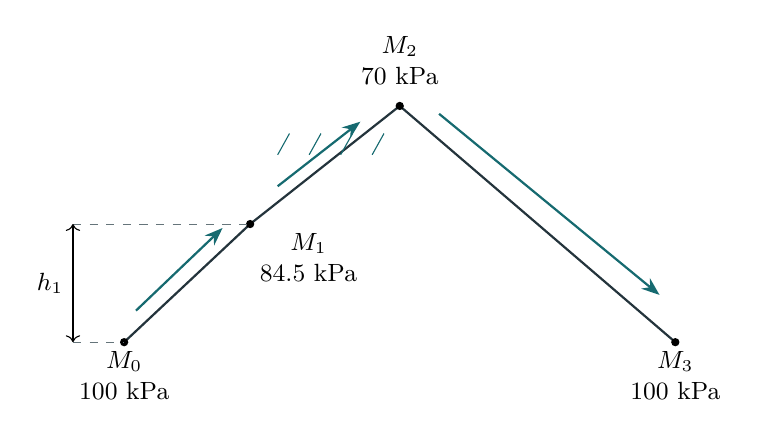
\begin{tikzpicture}[x=1cm,y=1cm]
\draw[object] (0,0)--(1.6,1.5)--(3.5,3)--(7,0);
\draw[motion] (.15,.4)--(1.25,1.45);
\draw[motion] (1.95,1.98)--(3,2.8);
\draw[motion] (4,2.9)--(6.8,.6);
\fill (0,0) circle(1.5pt) (1.6,1.5) circle(1.5pt) (3.5,3) circle(1.5pt) (7,0) circle(1.5pt);
\node[below,align=center] at (0,0) {$M_0$\\100 kPa};
\node[below right,align=center] at (1.6,1.5) {$M_1$\\84.5 kPa};
\node[above,align=center] at (3.5,3.15) {$M_2$\\70 kPa};
\node[below,align=center] at (7,0) {$M_3$\\100 kPa};
\draw[guide] (-.65,0)--(0,0) (-.65,1.5)--(1.6,1.5);
\draw[<->] (-.65,0)--(-.65,1.5) node[midway,left] {$h_1$};
\foreach \x in {2.1,2.5,2.9,3.3}{\draw[accent] (\x,2.65)--(\x-.15,2.38);}
\end{tikzpicture}\figcaption{图 热2.14　迎风侧成云降雨，背风侧按干绝热下沉估算。}\end{minipage}\end{center}

\workarea

\clearpage

\pdfbookmark[2]{第 15 题 U形管水银振动与封闭空气绝热弹性}{q15}

\section*{第 15 题\quad U形管水银振动与封闭空气绝热弹性}

等截面竖直U形管两端开口，管内水银全长$h$。压低一侧水银面，静止后撤去外压，忽略摩擦。证明振动周期$T_1=2\pi\sqrt{h/(2g)}$。再在两液面等高、气压等于大气压时封闭右端，封闭空气柱长$L$。气体作准静态绝热过程，水银作微小振动，证明
\[T_2=2\pi\sqrt{\frac{h}{g(2+\gamma h_0/L)}},\qquad \gamma=\frac{2L}{h_0}\left(\frac{T_1^2}{T_2^2}-1\right).\]
其中$h_0$为大气压对应的水银柱高度。

\begin{center}\begin{minipage}{0.96\linewidth}\centering
\begin{tikzpicture}[x=.9cm,y=.8cm]
\begin{scope}
\fill[accent!20] (0,0) rectangle (.7,1.8);
\fill[accent!20] (2.3,0) rectangle (3,1.2);
\fill[accent!20] (0,0) rectangle (3,.4);
\draw[object] (0,3.5)--(0,0)--(3,0)--(3,3.5);
\draw[object] (.7,3.5)--(.7,.4)--(2.3,.4)--(2.3,3.5);
\draw[guide] (-.4,1.5)--(3.4,1.5);
\draw[<->] (-.3,1.5)--(-.3,1.8) node[left,midway] {$y$};
\draw[<->] (3.35,1.2)--(3.35,1.5) node[right,midway] {$y$};
\node at (1.5,.2) {汞};
\node[above] at (.35,3.5) {$p_0$};
\node[above] at (2.65,3.5) {$p_0$};
\node[below] at (1.5,-.55) {两端开口};
\end{scope}
\begin{scope}[xshift=6.2cm]
\fill[accent!20] (0,0) rectangle (.7,1.8);
\fill[accent!20] (2.3,0) rectangle (3,1.2);
\fill[accent!20] (0,0) rectangle (3,.4);
\draw[object] (0,3.5)--(0,0)--(3,0)--(3,3.5);
\draw[object] (.7,3.5)--(.7,.4)--(2.3,.4)--(2.3,3.5);
\draw[guide] (-.4,1.5)--(3.4,1.5);
\draw[<->] (-.3,1.5)--(-.3,1.8) node[left,midway] {$y$};
\draw[<->] (3.35,1.2)--(3.35,1.5) node[right,midway] {$y$};
\node at (1.5,.2) {汞};
\draw[object] (2.3,3.5)--(3,3.5);
\draw[guide] (3,2.6)--(3.55,2.6);
\node[anchor=west,align=left] at (3.7,2.6) {封闭空气\\$L+y,\ p(y)$};
\node[above] at (.35,3.5) {$p_0$};
\node[below] at (1.5,-.55) {右端封闭};
\end{scope}
\end{tikzpicture}\figcaption{图 热2.15　以两液面等高的位置为$y=0$；左面升$y$时右面降$y$。}\end{minipage}\end{center}

\workarea

\clearpage

\pdfbookmark[2]{第 16 题 由声速驻波判断碘蒸气分子类型}{q16}

\section*{第 16 题\quad 由声速驻波判断碘蒸气分子类型}

在$400\,\mathrm K$的碘蒸气管中，用$1000\,\mathrm{Hz}$声波形成驻波，相邻波节间距6.77 cm。碘原子相对原子质量127。按理想气体模型判断蒸气分子是单原子还是双原子。给定声速$v=1/\sqrt{\rho K_s}$，其中$K_s=-V^{-1}(\dd V/\dd p)_{\mathrm{ad}}$为绝热压缩系数。

\begin{center}\begin{minipage}{0.96\linewidth}\centering
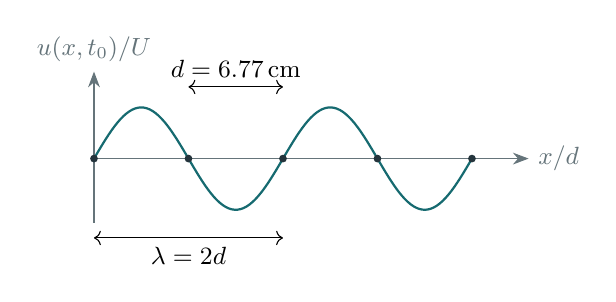
\begin{tikzpicture}[x=1.2cm,y=.65cm]
\draw[axis] (0,0)--(4.6,0) node[right] {$x/d$};
\draw[axis] (0,-1.25)--(0,1.7) node[above] {$u(x,t_0)/U$};
\draw[traj,domain=0:4,samples=130] plot (\x,{sin(180*\x)});
\foreach \x in {0,1,2,3,4}{\fill[ink] (\x,0) circle(1.4pt);}
\draw[<->] (1,1.4)--(2,1.4) node[midway,above] {$d=6.77\,\mathrm{cm}$};
\draw[<->] (0,-1.55)--(2,-1.55) node[midway,below] {$\lambda=2d$};
\end{tikzpicture}\figcaption{图 热2.16　相邻波节间距为半波长；曲线表示固定时刻的位移。}\end{minipage}\end{center}

\workarea

\clearpage

\pdfbookmark[2]{第 17 题 两个三角循环效率的比较}{q17}

\section*{第 17 题\quad 两个三角循环效率的比较}

定容摩尔热容量$C_V$恒定的理想气体经历图示两个顺时针三角循环$A_iB_iC_iA_i$（$i=1,2$）。两循环共用体积端点$V_1,V_2$；$A_iB_i$为过原点的直线$p=k_iV$，$B_iC_i$等容降压，$C_iA_i$等压压缩。比较效率$\eta_1,\eta_2$。

\begin{center}\begin{minipage}{0.96\linewidth}\centering
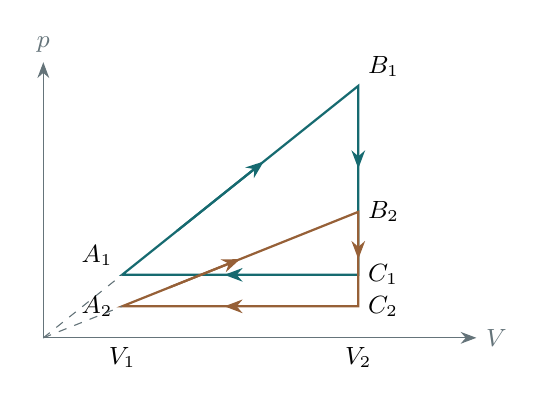
\begin{tikzpicture}[x=1cm,y=1cm,font=\small]\draw[axis] (0,0)--(5.5,0) node[right] {$V$};\draw[axis] (0,0)--(0,3.5) node[above] {$p$};
\draw[traj] (1,.8)--(4,3.2)--(4,.8)--cycle;\draw[warm,thick] (1,.4)--(4,1.6)--(4,.4)--cycle;\draw[guide] (0,0)--(1,.8);\draw[guide] (0,0)--(1,.4);\node[below] at (1,0){$V_1$};\node[below] at (4,0){$V_2$};\node[above left] at (1,.8){$A_1$};\node[above right] at (4,3.2){$B_1$};\node[right] at (4,.8){$C_1$};\node[left] at (1,.4){$A_2$};\node[right] at (4,1.6){$B_2$};\node[right] at (4,.4){$C_2$};
\draw[motion] (1.7,1.36)--(2.8,2.24);
\draw[motion] (4,2.8)--(4,2.15);
\draw[motion] (3.2,.8)--(2.3,.8);
\draw[motion,color=warm] (1.6,.64)--(2.5,1);
\draw[motion,color=warm] (4,1.4)--(4,1);
\draw[motion,color=warm] (3.2,.4)--(2.3,.4);
\end{tikzpicture}\figcaption{图 热2.17　同一体积端点下，两循环的压力尺度不同。}\end{minipage}\end{center}

\workarea

\clearpage

\pdfbookmark[2]{第 18 题 多条过程线构成循环的效率比较}{q18}

\section*{第 18 题\quad 多条过程线构成循环的效率比较}

理想气体的$C_V$为常量。图中两曲线为不同绝热线，三条直线的延长线过原点：12在$p=k_3V$上，34在$p=k_2V$上，56在$p=k_1V$上，$k_3>k_2>k_1>0$。1、3、5在同一绝热线上，2、4、6在另一线上。比较$\eta_{12431}$与$\eta_{12651}$；当三射线在同一参考体积处的压强比$p_1^*:p_2^*:p_3^*=1:2:3$时，再比较$\eta_{12431}$与$\eta_{34653}$。

\begin{center}\begin{minipage}{0.96\linewidth}\centering
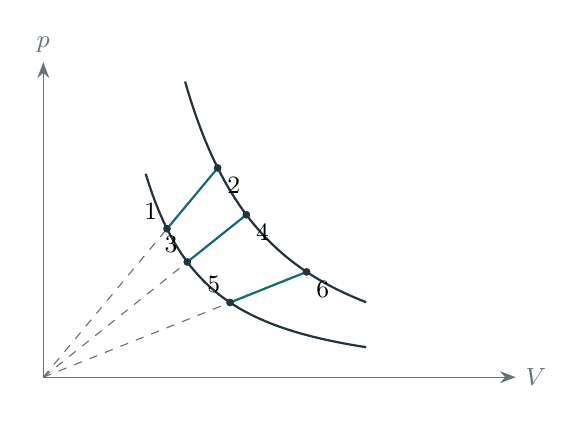
\begin{tikzpicture}[x=1cm,y=1cm,font=\small]\draw[axis] (0,0)--(6,0) node[right] {$V$};\draw[axis] (0,0)--(0,4) node[above] {$p$};
\draw[ink,thick,domain=1.3:4.1,samples=65] plot (\x,{4/pow(\x,5/3)});
\draw[ink,thick,domain=1.8:4.1,samples=65] plot (\x,{10/pow(\x,5/3)});
\draw[guide] (0,0)--(1.5706504008343012,1.8847804810011612);\draw[traj] (1.5706504008343012,1.8847804810011612)--(2.2146598521303114,2.6575918225563737);\fill[ink] (1.5706504008343012,1.8847804810011612) circle(1.4pt);\node[above left] at (1.5706504008343012,1.8847804810011612) {1};
\fill[ink] (2.2146598521303114,2.6575918225563737) circle(1.4pt);\node[below right] at (2.2146598521303114,2.6575918225563737) {2};
\draw[guide] (0,0)--(1.8285790999795744,1.4628632799836596);\draw[traj] (1.8285790999795744,1.4628632799836596)--(2.5783463443031147,2.0626770754424917);\fill[ink] (1.8285790999795744,1.4628632799836596) circle(1.4pt);\node[above left] at (1.8285790999795744,1.4628632799836596) {3};
\fill[ink] (2.5783463443031147,2.0626770754424917) circle(1.4pt);\node[below right] at (2.5783463443031147,2.0626770754424917) {4};
\draw[guide] (0,0)--(2.371373705661655,0.9485494822646621);\draw[traj] (2.371373705661655,0.9485494822646621)--(3.34370152488211,1.337480609952844);\fill[ink] (2.371373705661655,0.9485494822646621) circle(1.4pt);\node[above left] at (2.371373705661655,0.9485494822646621) {5};
\fill[ink] (3.34370152488211,1.337480609952844) circle(1.4pt);\node[below right] at (3.34370152488211,1.337480609952844) {6};

\end{tikzpicture}\figcaption{图 热2.18　两条绝热线与三条过原点射线相交；点号按循环路径排列。}\end{minipage}\end{center}

\workarea

\clearpage

\pdfbookmark[2]{第 19 题 氦气三直线循环效率}{q19}

\section*{第 19 题\quad 氦气三直线循环效率}

1 mol氦气视为单原子理想气体，经历三直线组成的顺时针循环$ABCA$：$A(2V_1,p_1)$、$B(V_1,p_1)$、$C(V_1,2p_1)$。求循环效率，并确定CA上的吸放热转折点；说明该转折点与绝热线相切的关系。

\begin{center}\begin{minipage}{0.96\linewidth}\centering
\begin{tikzpicture}[x=3cm,y=1.7cm]
\draw[axis] (0,0)--(2.8,0) node[right] {$V/V_1$};
\draw[axis] (0,0)--(0,2.9) node[above] {$p/p_1$};
\draw[traj] (2,1)--(1,1)--(1,2)--cycle;
\draw[motion] (1.8,1)--(1.3,1);
\draw[motion] (1,1.2)--(1,1.7);
\draw[motion] (1.2,1.8)--(1.55,1.45);
\fill (2,1) circle(1.5pt) node[below right] {$A$};
\fill (1,1) circle(1.5pt) node[below left] {$B$};
\fill (1,2) circle(1.5pt) node[above left] {$C$};
\foreach \u in {1,2}{\draw (\u,.03)--(\u,-.03) node[below] {$\u$};}
\foreach \u in {1,2}{\draw (.02,\u)--(-.02,\u) node[left] {$\u$};}
\end{tikzpicture}\figcaption{图 热2.19　AB等压压缩，BC等容升温，CA沿负斜率直线膨胀。}\end{minipage}\end{center}

\workarea

\clearpage

\pdfbookmark[2]{第 20 题 直线加绝热线循环的效率与极值温度}{q20}

\section*{第 20 题\quad 直线加绝热线循环的效率与极值温度}

0.1 mol单原子理想气体从$I(V_0=8.00\,\mathrm{m^3},p_0=32.0\,\mathrm{Pa})$沿直线到$F(V_1=64.0\,\mathrm{m^3},p_1=1.0\,\mathrm{Pa})$，再沿准静态绝热线回到I。求循环效率及全过程的最高、最低温度。

\begin{center}\begin{minipage}{0.96\linewidth}\centering
\begin{tikzpicture}[x=1cm,y=1cm,font=\small]\draw[axis] (0,0)--(6,0) node[right] {$V/\mathrm{m^3}$};\draw[axis] (0,0)--(0,4) node[above] {$p/\mathrm{Pa}$};
\draw[traj] (.64,3.2)--(5.12,.1);\draw[warm,thick,domain=.64:5.12,samples=90] plot (\x,{3.2*pow(.64/\x,5/3)});\fill[ink] (0.64,3.2) circle(1.4pt);\node[above right] at (0.64,3.2) {I};
\fill[ink] (5.12,0.1) circle(1.4pt);\node[above right] at (5.12,0.1) {F};

\draw[motion] (1.4,2.6741071429)--(2.1,2.1897321429);
\draw[motion,color=warm,domain=3.8:3.1,samples=25]
 plot (\x,{3.2*pow(.64/\x,5/3)});
\end{tikzpicture}\figcaption{图 热2.20　直线膨胀后沿绝热线压缩回I；图中体积按0.08 cm/m$^3$缩放。}\end{minipage}\end{center}

\workarea

\clearpage

\pdfbookmark[2]{第 21 题 圆形准静态循环的功、热量和转折点}{q21}

\section*{第 21 题\quad 圆形准静态循环的功、热量和转折点}

1 mol单原子理想气体沿图示顺时针圆形循环ABCDA运行。归一化坐标$x=V/V_0$、$y=p/p_0$满足$(x-2)^2+(y-2)^2=1$，$p_0=10^5\,\mathrm{Pa}$、$V_0=10^{-3}\,\mathrm{m^3}$，A、B、C、D为左、上、右、下四端点。求：一周对外功；ABC的内能增量；ABC的代数吸热量；吸放热转折点坐标应满足的代数方程（不必求解）。

\begin{center}\begin{minipage}{0.96\linewidth}\centering
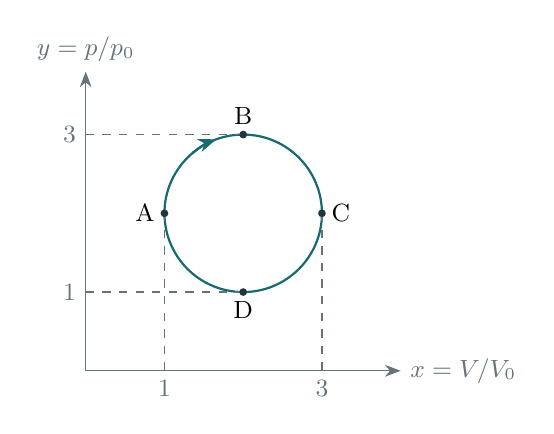
\begin{tikzpicture}[x=1cm,y=1cm,font=\small]\draw[axis] (0,0)--(4,0) node[right] {$x=V/V_0$};\draw[axis] (0,0)--(0,3.8) node[above] {$y=p/p_0$};
\draw[traj] (2,2) circle(1);\draw[guide] (1,0) node[below]{1}--(1,2);\draw[guide] (3,0) node[below]{3}--(3,2);\draw[guide] (0,1) node[left]{1}--(2,1);\draw[guide] (0,3) node[left]{3}--(2,3);\fill[ink] (1,2) circle(1.4pt);\node[left] at (1,2) {A};
\fill[ink] (2,3) circle(1.4pt);\node[above] at (2,3) {B};
\fill[ink] (3,2) circle(1.4pt);\node[right] at (3,2) {C};
\fill[ink] (2,1) circle(1.4pt);\node[below] at (2,1) {D};
\draw[motion] ({2+cos(130)},{2+sin(130)}) arc(130:110:1);
\end{tikzpicture}\figcaption{图 热2.21　归一化坐标内为半径1的圆，箭头沿A、B、C、D依次运行。}\end{minipage}\end{center}

\workarea

\clearpage

\pdfbookmark[2]{第 22 题 可逆卡诺空调的维持室温与最高外温}{q22}

\section*{第 22 题\quad 可逆卡诺空调的维持室温与最高外温}

一台理想空调按可逆卡诺循环运行，连续工作时输入功率$P_0$。夏季室外恒温$T_1$，连续工作可维持室温$T_2$；室外向室内的漏热功率为$A(T_1-T_2)$。求$T_2$关于$T_1,P_0,A$的表达式。已知室外30℃时，空调只有30\%时间工作即可维持室内20℃；求连续工作仍能维持20℃的最高室外温度。冬季反向运行作为热泵，求仍可维持20℃的最低室外温度。绝对零度取$-273^\circ\mathrm C$。

\begin{center}\begin{minipage}{0.96\linewidth}\centering
\begin{tikzpicture}[x=1cm,y=1cm,font=\small]\node[draw,align=center] (room) at (0,0){室内\\$T_2$};\node[draw,align=center] (ac) at (3,0){空调\\可逆循环};\node[draw,align=center] (out) at (6,0){室外\\$T_1$};\draw[force] (3,-1.5)--(ac) node[pos=0,below]{$P_0$};\draw[motion] (room)--(ac) node[midway,above]{$\dot Q_c$};\draw[motion] (ac)--(out) node[midway,above]{$\dot Q_h$};\draw[force] (6,1.2)--(0,1.2) node[midway,above]{漏热$A(T_1-T_2)$};
\end{tikzpicture}\figcaption{图 热2.22　夏季空调从室内吸热，房屋传热则从室外流向室内。}\end{minipage}\end{center}

\workarea

\clearpage

\pdfbookmark[2]{第 23 题 绝热细棒热平衡过程的熵增}{q23}

\section*{第 23 题\quad 绝热细棒热平衡过程的熵增}

均匀细棒长$l$，线密度$\lambda$，比热$c$恒定；初始两端温度$T_1$、$2T_1$，中间温度线性分布。棒对外绝热，最终达到热平衡，不作外功。求棒的总熵增量，并判断过程是否可逆。

\begin{center}\begin{minipage}{0.96\linewidth}\centering
\begin{tikzpicture}[x=1cm,y=1cm,font=\small]\draw[axis] (0,0)--(5.6,0) node[right] {$x$};\draw[axis] (0,0)--(0,3) node[above] {$T$};
\draw[traj] (0,1)--(5,2);\node[left] at (0,1){$T_1$};\node[left] at (0,2){$2T_1$};\draw[guide] (0,2)--(5,2);\node[below] at (5,0){$l$};
\end{tikzpicture}\figcaption{图 热2.23　初始温度沿棒长线性增加，棒整体对外绝热。}\end{minipage}\end{center}

\workarea

\clearpage

\pdfbookmark[2]{第 24 题 氧气复合循环效率与 S-T 图像}{q24}

\section*{第 24 题\quad 氧气复合循环效率与 S-T 图像}

3.2 g氧气，$\gamma=7/5$，从状态1（$p_1=1.0\,\mathrm{atm},V_1=1.0\,\mathrm L$）等压膨胀到2（$V_2=2.0\,\mathrm L$），再等容升压到3（$p_3=2.0\,\mathrm{atm}$），再准静态绝热膨胀到4（$T_4=T_1$），最后等温压缩回1。求循环效率。取熵S为纵轴、温度T为横轴，画出形状正确的$S-T$图，标各特征点坐标，以$S_1$表示初态熵。各传热段按内部可逆过程计算。

\begin{center}\begin{minipage}{0.96\linewidth}\centering
\begin{tikzpicture}[x=1.45cm,y=1.65cm,font=\small]
\draw[axis] (-.25,0)--(4.8,0) node[right] {$u=\ln(V/V_1)$};
\draw[axis] (0,0)--(0,2.6) node[above] {$p/\mathrm{atm}$};
\draw[traj] (0,1)--({ln(2)},1)--({ln(2)},2);
\draw[warm,thick,domain=ln(2):ln(64),samples=100]
 plot (\x,{2*exp(-1.4*(\x-ln(2)))});
\draw[traj,domain=0:ln(64),samples=100] plot (\x,{exp(-\x)});
\fill (0,1) circle(1.5pt) node[left] {1};
\fill ({ln(2)},1) circle(1.5pt) node[below right] {2};
\fill ({ln(2)},2) circle(1.5pt) node[above right] {3};
\fill ({ln(64)},.015625) circle(1.5pt) node[above right] {4};
\draw[guide] ({ln(2)},0) node[below] {$\ln2$}--({ln(2)},.85);
\node[below] at ({ln(64)},0) {$\ln64$};
\draw[motion] (.12,1)--(.48,1);
\draw[motion] ({ln(2)},1.2)--({ln(2)},1.7);
\draw[motion,warm,domain=1:1.5,samples=30]
 plot (\x,{2*exp(-1.4*(\x-ln(2)))});
\draw[motion,domain=3.1:2.5,samples=30] plot (\x,{exp(-\x)});

\end{tikzpicture}\figcaption{图 热2.24　体积坐标为 $u=\ln(V/V_A)$，沿曲线的功按 $W=\int pV\dd u$ 计算。}\end{minipage}\end{center}

\workarea

\clearpage

\pdfbookmark[2]{第 25 题 由 T-S 直线导出理想气体过程方程}{q25}

\section*{第 25 题\quad 由 T-S 直线导出理想气体过程方程}

$\nu$ mol理想气体，$\gamma$恒定，经历图示准静态过程：$T-S$图中两点$(S_1,T_1)$、$(S_2,T_2)$之间为直线，$T_2>T_1>0$、$S_2>S_1$。导出过程方程。在可逆情形下，可由 $\delta Q=T\dd S$ 求过程热容量。状态轨迹也可直接由理想气体的熵微分确定。

\begin{center}\begin{minipage}{0.96\linewidth}\centering
\begin{tikzpicture}[x=1cm,y=1cm,font=\small]\draw[axis] (0,0)--(5,0) node[right] {$S$};\draw[axis] (0,0)--(0,3.8) node[above] {$T$};
\draw[traj] (1,1)--(4,3);\fill[ink] (1,1) circle(1.4pt);\node[above left] at (1,1) {$(S_1,T_1)$};
\fill[ink] (4,3) circle(1.4pt);\node[above right] at (4,3) {$(S_2,T_2)$};
\draw[motion] (2,1.667)--(3,2.333);
\end{tikzpicture}\figcaption{图 热2.25　熵作横轴、温度作纵轴；直线斜率为$1/m$。}\end{minipage}\end{center}

\workarea

\end{document}
